\documentclass[11pt,a4paper]{article}
\usepackage[margin=2.2cm]{geometry}
\usepackage{amsmath,amssymb}
\usepackage{graphicx}
\usepackage{booktabs}
\usepackage{float}
\usepackage[hidelinks]{hyperref}
\usepackage{xcolor}
\usepackage{caption}
\captionsetup[table]{skip=8pt}
\newcommand{\pending}[1]{\textcolor{red!70!black}{[pending: #1]}}

\title{Direction-aware residual weighting for physics-informed neural networks:\\
a matrix generalization of regime-aware time weighting}
\author{Chandragupt Sharma}
\date{Interim report, 22--23 November 2026}

\begin{document}
\maketitle

\begin{abstract}
Turinici's regime-aware time weighting (arXiv:2407.21642v2) weights the residual of a
physics-informed neural network (PINN) in time, using one growth rate per time and
hence the same weight for every direction of the residual. We extend his minimax
argument to a matrix weight per time, built from the tangent propagator of the ODE:
$W(t)\propto G(t)/\sqrt{\operatorname{tr}G(t)}$ with
$G(t)=\int_t^T\Phi(s,t)^{\top}\Phi(s,t)\,ds$. Turinici's weight is the
direction-blind special case, and the guaranteed improvement over the best
direction-blind weight is at most $\sqrt n$. The weight can be computed along the
PINN's own current path, without a reference solution. In pre-registered experiments
on Rössler and Lorenz-96, the matrix weight beat the direction-blind version of the
same weight, uniform weighting and Turinici's weighting. On Rössler over $[0,10]$, 30 of
36 networks stayed accurate with the matrix weight, against 13, 4 and 1 of 36 for the
other three. The final-time error was 76 times lower than with uniform weighting. On
Lorenz-63 driving up to 29 damped modes, the matrix weight kept 27 of 36 networks
accurate at every dimension, while the direction-blind version fell to 5 of 36. On plain
Lorenz-63 the benefit is mostly an automatic causal time schedule. There, the
direction-blind Gramian weight and well-tuned causal weighting do about as well, and
on easy problems the matrix weight costs a little accuracy.
\end{abstract}

\section{Summary of findings}
\begin{enumerate}
\item \textbf{Where the plain loss fails, weights from the tangent Gramian fix training.} On
  Lorenz-63 windows of length 1, uniform weighting kept 7 of 36 networks accurate and
  Turinici's weighting 5 of 36. The Gramian weights computed along the PINN's own path
  kept 24 (scalar) to 27 (matrix), with about 100 times lower median error. The failures
  of the uniform and Turinici losses persisted with 2.5 times more steps, a wider network
  and a denser grid.
\item \textbf{The direction effect grows with the number of harmless directions.}
  \begin{itemize}
  \item Matrix against direction-blind weight, same Gramian, self-consistent: Rössler over $[0,10]$, 25 times lower error; Lorenz-96 over $[0,1]$, 2.5 times lower.
  \item Lorenz-63 driving $k$ damped modes: 2, 8, 50 and 100 times lower error at $k=0,3,9,29$.
  \item Plain Lorenz-63 with self-consistent weights: no reliable difference.
  \end{itemize}
\item \textbf{Mechanism.} Matrix-weighted networks leave 60--73\% of their leftover residual
  along the direction the dynamics erase fastest. Uniformly weighted networks put about
  60\% along the most harmful direction.
\item \textbf{Limits.}
  \begin{itemize}
  \item On easy two-dimensional problems, the matrix weight gives 1.2 to 4 times larger errors.
  \item A single Lorenz-63 window of length 2 remains out of reach for every method.
  \item Weighting for the final-time error alone (Turinici's target) fails beyond $T=0.5$.
  \item For long horizons, short time-marching segments with uniform weighting stay the most reliable.
  \item The matrix weight costs about three times the GPU time of uniform weighting per run.
  \end{itemize}
\end{enumerate}

\begin{table}[H]\centering
\caption{Pre-registered hypotheses and verdicts (rules in \texttt{docs/plan.md}, fixed before training).}
\small
\begin{tabular}{p{4.6cm}p{1.1cm}p{4.2cm}p{4.6cm}}\toprule
Hypothesis & Gate & Systems & Verdict\\\midrule
H1 mechanism, known directions & 0 & stiff saddle, Davis--Skodje & partial\\
H2 usable method & 1 & Lorenz-63, $T\in\{0.5,1,2\}$ & \pending{CPU runs; GPU replicate gives partial}\\
H3 gain over uniform grows with dimension & 2 & Lorenz-63 with $k$ damped modes & not supported\\
H4 same rule on further systems & 3 & Rössler, Lorenz-96 & \textbf{supported for both}\\\bottomrule
\end{tabular}
\end{table}

\section{Method}
\subsection{From scalar to matrix weights}
For an ODE $\dot x=f(x)$ and a PINN $\hat x(t)$ with exact initial state, write the
residual as $r=\dot{\hat x}-f(\hat x)$. To first order, the error $e=x-\hat x$ satisfies
$\dot e=J(t)e-r$, so
\[
 e(t)=-\int_0^t\Phi(t,s)\,r(s)\,ds .
\]
Here $\Phi$ is the tangent propagator. By Minkowski's inequality,
\[
 \|e\|_{L^2(0,T)}\le\int_0^T\sqrt{r(s)^{\top}G(s)\,r(s)}\,ds,
 \qquad
 G(s)=\int_s^T\Phi(\tau,s)^{\top}\Phi(\tau,s)\,d\tau .
\]
The matrix $G(s)$ measures how much error a unit residual at time $s$ causes in each
direction over the rest of the window.

Following Turinici's Proposition 2, allow a matrix weight $M(s)\succeq0$ in the loss
$\int r^{\top}Mr$, with budget $\int\operatorname{tr}M=1$. Two Cauchy--Schwarz steps and
the trace inequality $\lambda_{\max}(M^{-1/2}GM^{-1/2})\ge\operatorname{tr}G/\operatorname{tr}M$
give the minimax-optimal weight
\[
 M^\star(s)\propto\frac{G(s)}{\sqrt{\operatorname{tr}G(s)}} .
\]
The best direction-blind weight is $\rho^\star(s)\propto\sqrt{\lambda_{\max}G(s)}$. The
ratio of the two guaranteed bounds lies in $[1,\sqrt n]$. Turinici's weight is the
direction-blind case built on a looser one-sided growth bound. Replacing $G$ by
$\Phi(T,s)^{\top}\Phi(T,s)$ gives the final-time version. The full derivation is in
\texttt{docs/theory.md}.

\subsection{Computing the weight}
Let the grid be $t_0,\dots,t_{N-1}$ with spacing $h$. With step propagators
$\Phi_i=\exp\!\big(h(J_i+J_{i+1})/2\big)$, the window Gramian follows from the backward
recursion
\[
 G_i=\Phi_i^{\top}G_{i+1}\Phi_i+\tfrac h2(I+\Phi_i^{\top}\Phi_i),\qquad G_{N-1}=0 .
\]
The Jacobians are taken along the reference solution (\emph{oracle}, labelled
\texttt{-orc}) or along the PINN's own current path, refreshed every 10 steps
(\emph{self-consistent}, \texttt{-self}). The self-consistent version needs no reference
solution, just as Turinici's Eq.~(17) uses the PINN's own state.

\subsection{Weights compared}
\begin{itemize}
\item \texttt{U}: uniform weighting.
\item \texttt{TUR}: Turinici's Eqs.~(13) and (17).
\item \texttt{S}: the best direction-blind weight, $\sqrt{\lambda_{\max}G}\,I$.
\item \texttt{M}: the matrix weight, $G/\sqrt{\operatorname{tr}G}$.
\item \texttt{D}: direction only, $nG/\operatorname{tr}G$, with the same total weight at every time.
\item Causal weighting (Wang, Sankaran and Perdikaris): $\rho_i\propto\exp(-\varepsilon h\sum_{j<i}\|r_j\|^2)$.
\end{itemize}
Every weight is rescaled to mean trace $n$.

\subsection{Experimental design}
\begin{itemize}
\item \textbf{Training.} Every network is a $4\times64$ tanh MLP with exact initial condition. Collocation is a fixed grid of 512 times. Training uses 20{,}000 Adam steps, with the learning rate decaying from $10^{-3}$ to $10^{-5}$, in float32.
\item \textbf{Fairness.} All methods share the networks, initializations, grid and budget; only the weights differ.
\item \textbf{Scale.} Each setting trains 36 networks per method: 12 attractor initial conditions $\times$ 3 seeds, or 8 $\times$ 3 for the two-dimensional systems.
\item \textbf{Statistics.} Contrasts are paired differences of $\log_{10}$ RMS trajectory error, averaged over seeds within each initial condition, with 95\% bootstrap intervals over initial conditions. ``A beats B'' requires at least 1.5 times lower error with the interval below zero.
\item \textbf{Pre-registration.} Hypotheses, rules and settings were committed before any training. Later additions were committed as dated amendments before their runs.
\item \textbf{Platforms.} Lorenz-63 ran on a CPU laptop; the other gates ran on Kaggle T4 GPUs. A complete GPU replicate of the Lorenz-63 runs reproduced the CPU success counts exactly.
\end{itemize}

\section{Results}
\subsection{Rössler and Lorenz-96 (Gate 3, H4 supported)}
\begin{table}[H]\centering
\caption{Gate 3. Success = trajectory error below 1 over the whole window, out of 36
networks. Errors are medians over the 36 networks.}
\begin{tabular}{llcccc}\toprule
System, window & Quantity & uniform & Turinici & scalar Gramian & \textbf{matrix}\\\midrule
Rössler, $[0,10]$ & success & 4 & 1 & 13 & \textbf{30}\\
 & final-time error & 3.19 & 5.61 & 5.60 & \textbf{0.042}\\
 & RMS error & 1.97 & 3.58 & 2.27 & \textbf{0.031}\\\midrule
Rössler, $[0,5]$ & success & 18 & 19 & 21 & \textbf{25}\\
 & final-time error & 0.216 & 0.240 & 0.023 & \textbf{0.0036}\\\midrule
Lorenz-96, $[0,1]$ & success & 29 & 13 & 36 & \textbf{36}\\
 & final-time error & 0.187 & 2.44 & 0.057 & \textbf{0.015}\\\midrule
Lorenz-96, $[0,2]$ & success & 0 & 0 & 1 & \textbf{10}\\
 & final-time error & 14.9 & 15.0 & 12.2 & \textbf{8.45}\\\bottomrule
\end{tabular}
\end{table}

\paragraph{Planned contrasts for the matrix weight.} These are fold changes in RMS error.
\begin{itemize}
\item \textbf{Rössler $T=10$.} Against scalar 0.04, uniform 0.03, Turinici 0.02; all three ``beats''.
\item \textbf{Rössler $T=5$.} Against uniform 0.17 and Turinici 0.16 (``beats''); against scalar 0.36 (no decision).
\item \textbf{Lorenz-96 $T=1$.} Against scalar 0.41, uniform 0.07, Turinici 0.02; all three ``beats''.
\item \textbf{Lorenz-96 $T=2$.} Against uniform 0.19 and Turinici 0.16 (``beats''); against scalar 0.42 (no decision).
\end{itemize}
The matrix weight never lost a contrast, so H4 is supported for both systems.

\begin{figure}[H]\centering
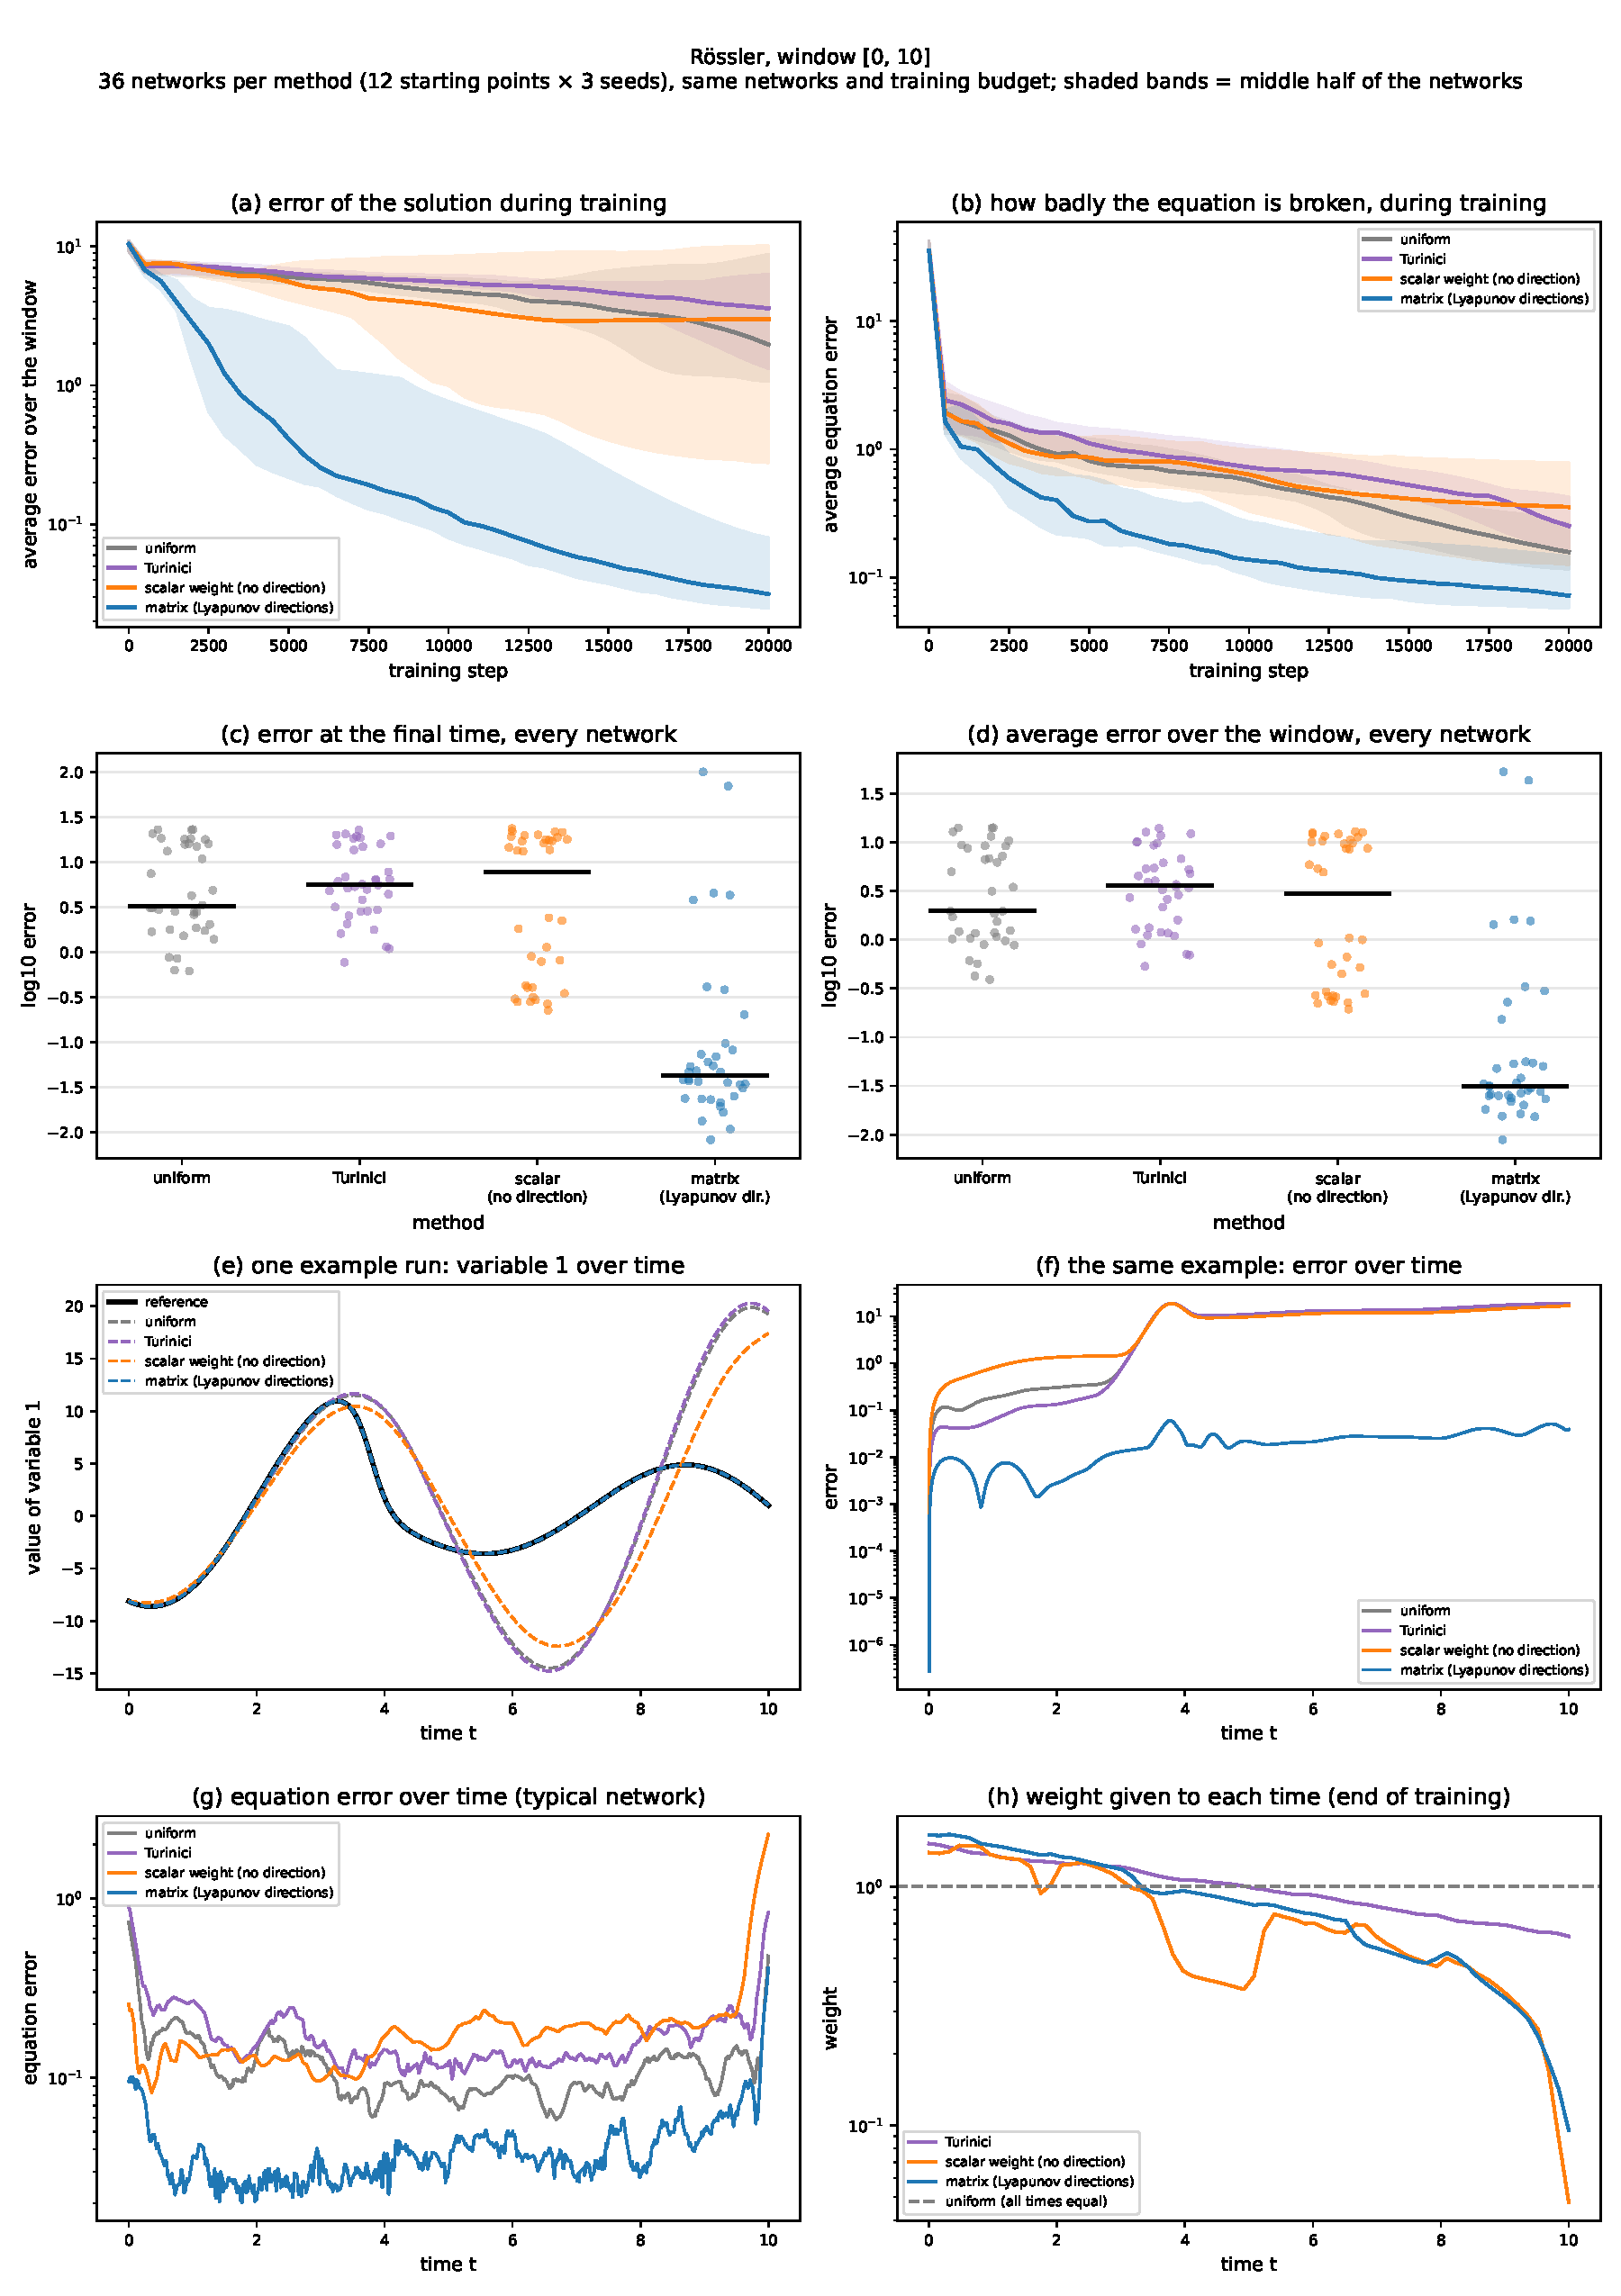
\includegraphics[width=\textwidth]{figures/turinici_style_rossler_T10.pdf}
\caption{Rössler over $[0,10]$, in the style of Turinici's figures. (a) Trajectory error and
(b) equation error during training (median and quartiles of 36 networks).
(c) Final-time error and (d) RMS error per network. (e) An example trajectory and
(f) its error; this is initial condition 1, seed 0, the same starting network for every
method. (g) Equation error over the window. (h) The learned time weights.}
\end{figure}

\begin{figure}[H]\centering
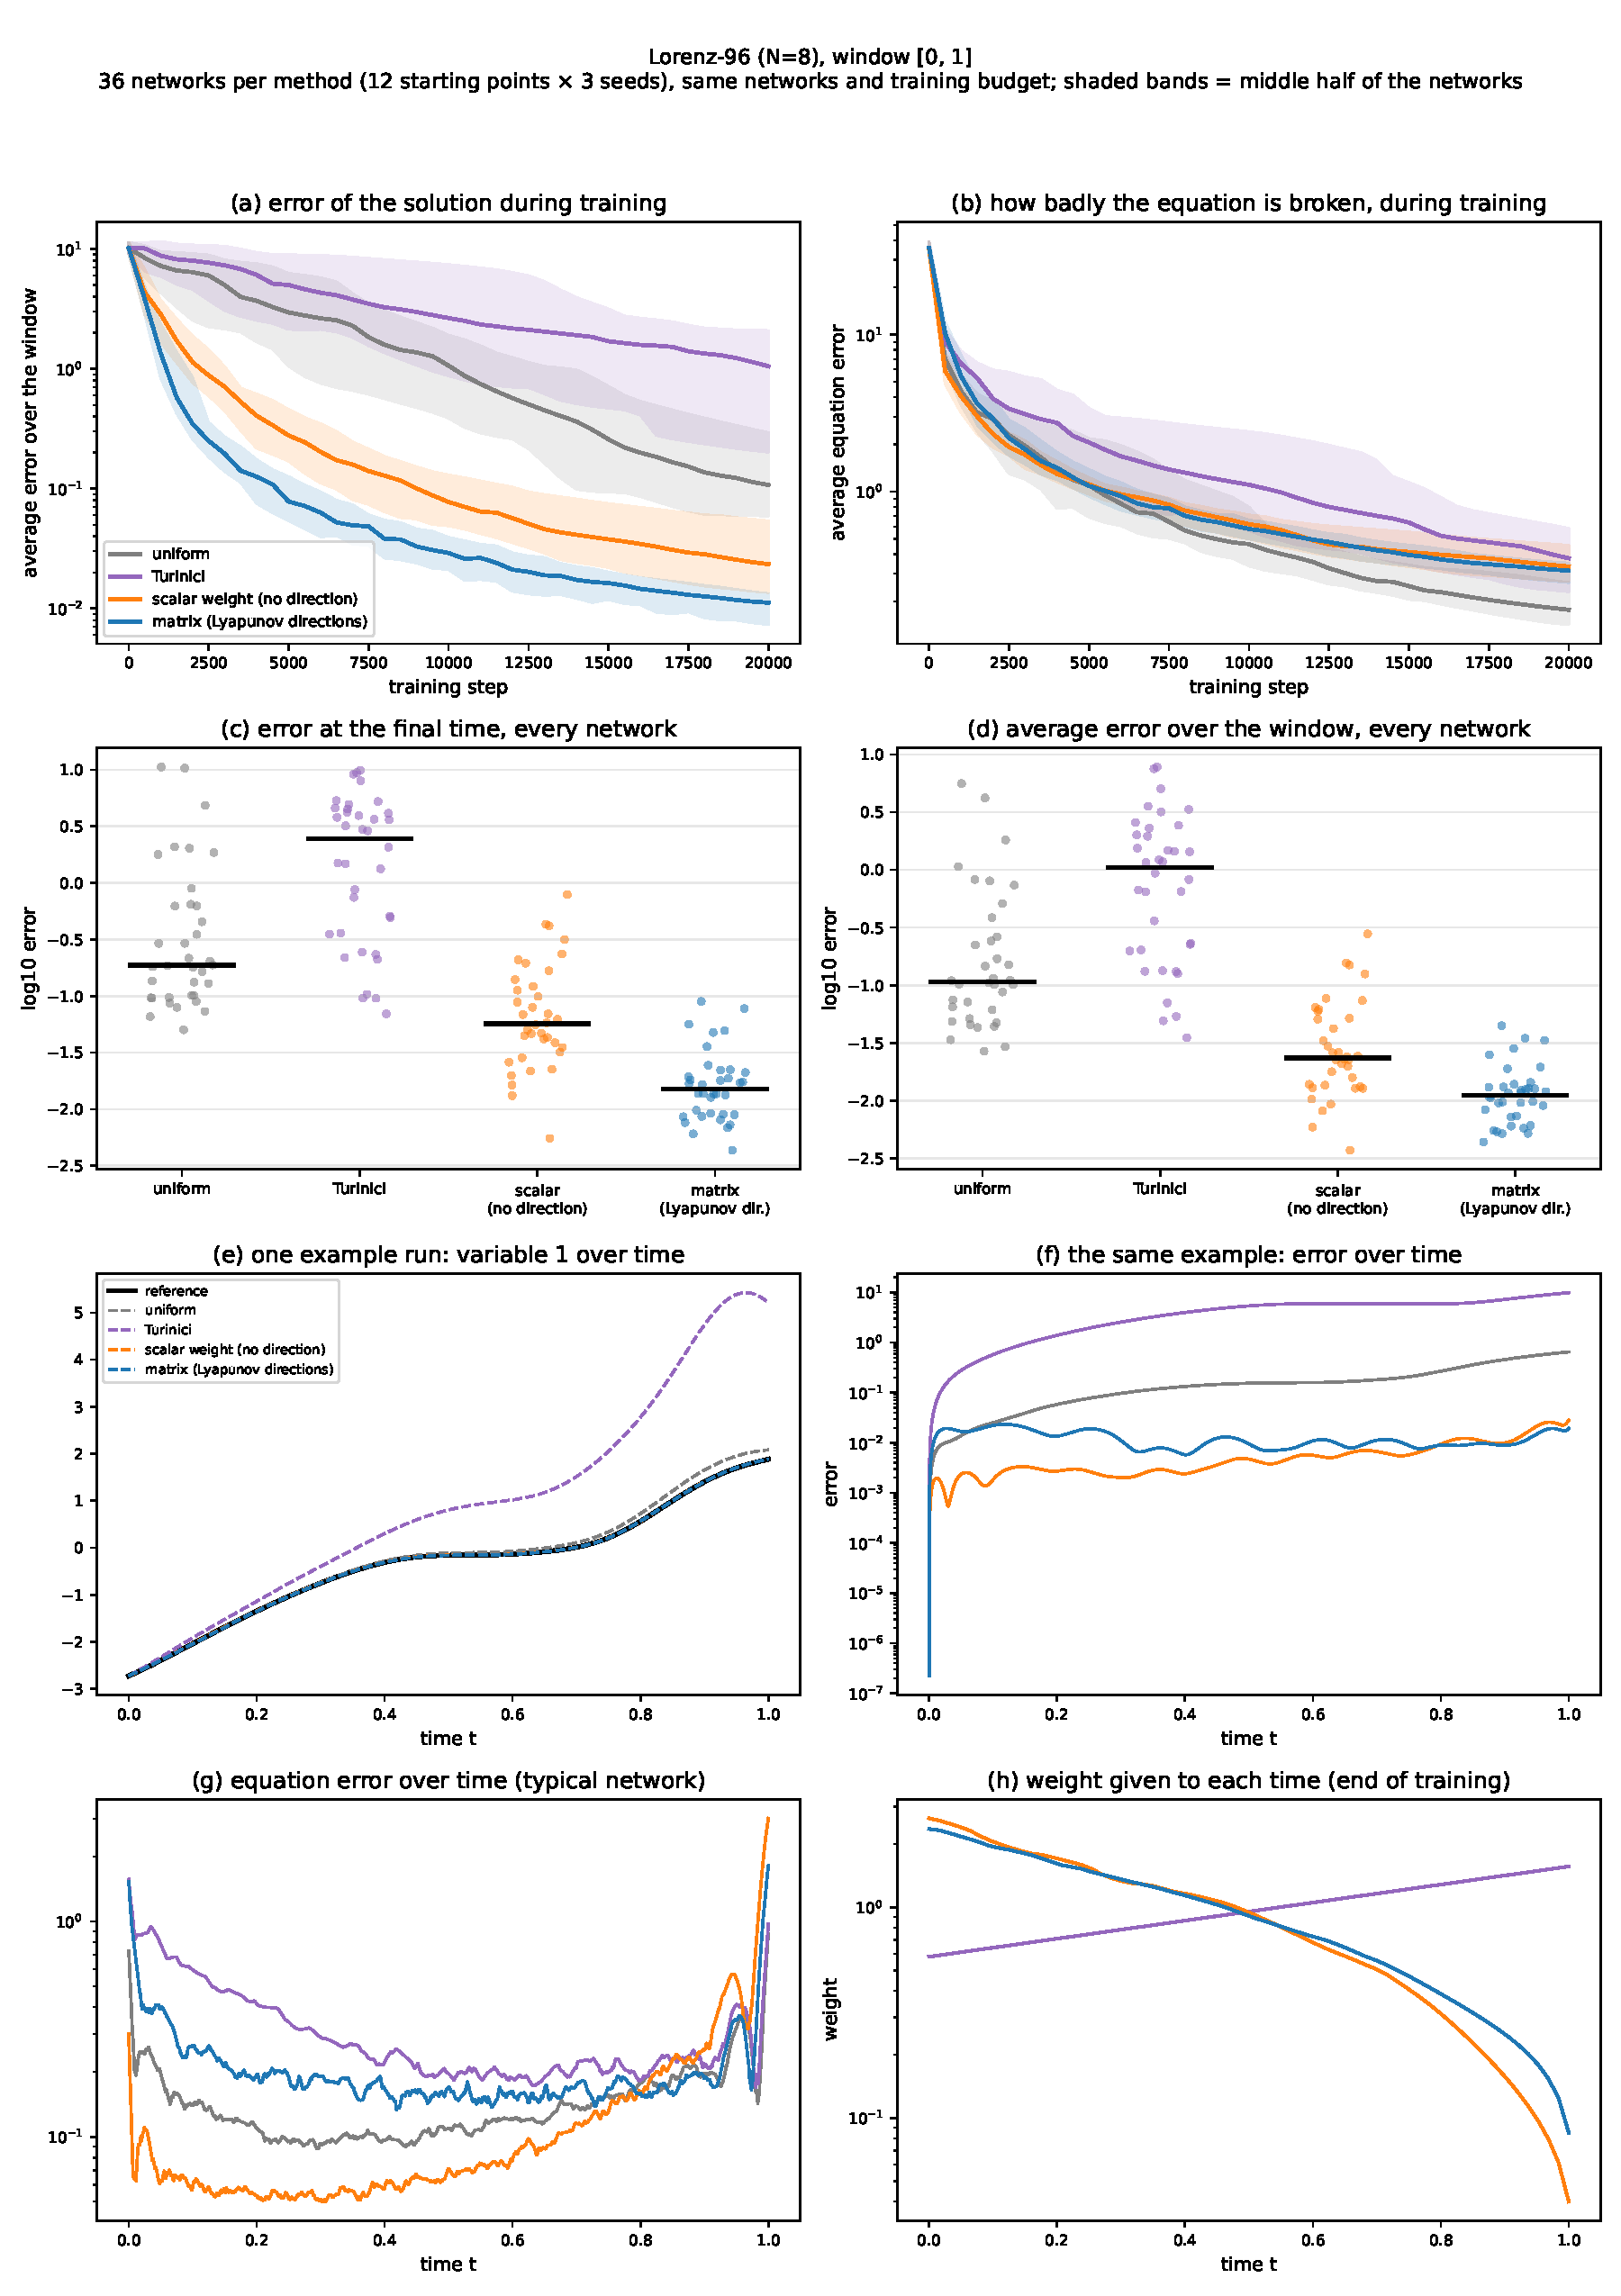
\includegraphics[width=\textwidth]{figures/turinici_style_lorenz96_n8_T1.pdf}
\caption{Lorenz-96 ($N=8$, $F=8$) over $[0,1]$. Panels as in the Rössler figure.}
\end{figure}

\subsection{Dimension dial: Lorenz-63 driving $k$ damped modes (Gate 2)}
\begin{table}[H]\centering
\caption{Gate 2: successes (out of 36) on the Lorenz part, window $[0,1]$.}
\begin{tabular}{lcccccc}\toprule
$k$ ($n=3+k$) & uniform & Turinici & scalar (orc.) & matrix (orc.) & scalar (self) & matrix (self)\\\midrule
0 & 7 & 5 & 9 & 23 & 24 & \textbf{27}\\
3 & 7 & 4 & 5 & 17 & 20 & \textbf{27}\\
9 & 3 & 0 & 4 & 10 & 7 & \textbf{27}\\
29 & 0 & 0 & 3 & 5 & 5 & \textbf{27}\\\bottomrule
\end{tabular}
\end{table}
The pre-registered H3 contrast, matrix against uniform, is already about 100-fold at
$k=0$ and does not grow reliably, so H3 is not supported. The contrast of the matrix
weight against the direction-blind scalar weight does grow with $k$: 0.52 (no decision),
then 0.13, 0.02 and 0.01. A direction-blind weight wastes more of its budget as more
directions become harmless, as the theory predicts.

\begin{figure}[H]\centering
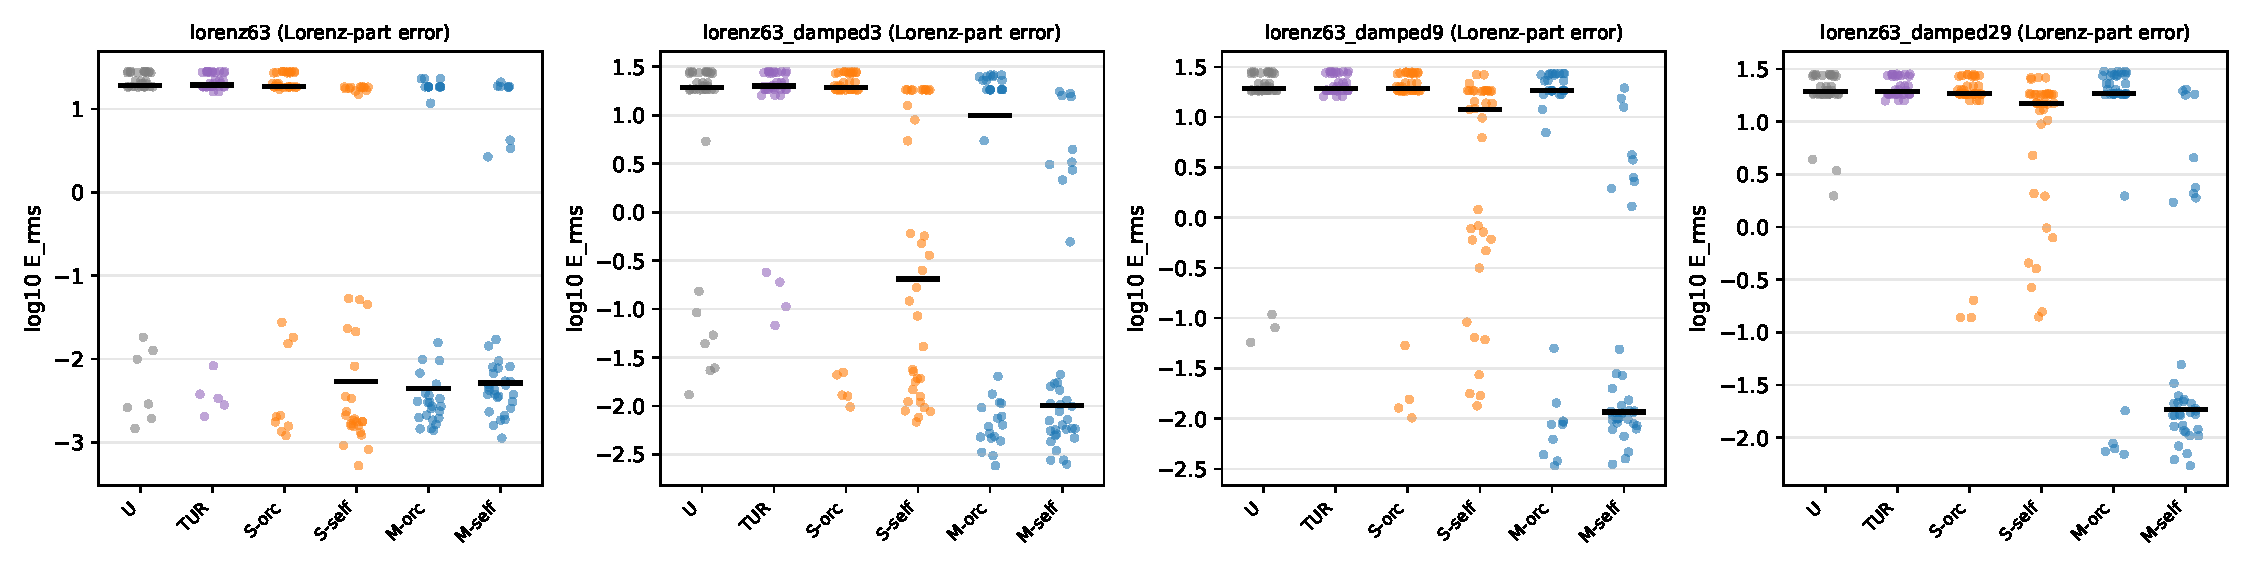
\includegraphics[width=\textwidth]{figures/gate2_errors.pdf}
\caption{Gate 2: RMS error on the Lorenz part, for every network and method.}
\end{figure}

\subsection{Plain Lorenz-63 (Gate 1)}
The GPU replicate is complete. The CPU runs that decide H2 are half complete and match
it exactly where both exist: at $T=1$ the successes are 27, 24, 23, 9, 7 and 5 for the
matrix (self), scalar (self), matrix (oracle), scalar (oracle), uniform and Turinici
weights respectively.
\begin{itemize}
\item \textbf{$T=0.5$.} All methods succeed.
\item \textbf{$T=1$.} The self-consistent weights beat uniform and Turinici by about 100-fold. The matrix and scalar versions do not differ reliably (fold change 0.52, interval includes 1).
\item \textbf{$T=2$.} Every method mostly fails. The matrix weight succeeds most often (8 of 36, against 0 for uniform and Turinici).
\end{itemize}
Applying the H2 rule to the replicate gives \emph{partial}. \pending{the decisive CPU
runs; about one hour.}

\paragraph{Causal weighting (side run).} With fixed $\varepsilon$:
\begin{itemize}
\item at $T=1$, successes were 20, 25 and 21 of 36 for $\varepsilon=0.1$, 1 and 10;
\item at $T=2$, successes were 0 to 3 of 36.
\end{itemize}
On plain Lorenz-63, well-tuned causal weighting is therefore about as good as the
Gramian weights. The training histories explain why. Early in training, the
self-consistent weights put very little weight on the late part of the window. This acts
as an automatic causal schedule, with no parameter to tune. \pending{causal weighting
($\varepsilon=1$) on Rössler, Lorenz-96 and the damped systems}

\subsection{Two-dimensional dial systems (Gate 0, H1 partial)}
Fold changes of the matrix (oracle) weight against the scalar (oracle) weight:
\begin{itemize}
\item stiff linear saddle, $\kappa=1,4,16,64$: 1.9, 3.1 and 4.3 (worse), then \textbf{0.50} (beats);
\item Davis--Skodje, $\gamma=3,6,18,66$: 1.2, 2.5 and 1.8 (worse), then 1.0 (no decision).
\end{itemize}
Every method succeeds on these easy problems. There, the matrix weight trades a little
accuracy for a larger residual along the contracting direction. It helps only at the
stiffest saddle. \pending{soft initial-condition check of this result}

\subsection{Further side runs}
\begin{itemize}
\item \textbf{Final-time matrix weight} (Turinici's target, $\Phi(T,t)^{\top}\Phi(T,t)$):
  21 and 20 successes at $T=0.5$, but 0--1 at $T\ge1$. The window target is what helps.
\item \textbf{Direction only} (same total weight at every time), Lorenz-63 $T=1$: 23 of 36
  (self-consistent) and 10 of 36 (oracle), against 7 for uniform.
\item \textbf{Time-marching to horizon 4} (Lorenz-63):
  \begin{itemize}
  \item segments of length 0.5: uniform 27, scalar 24, matrix 25 successes;
  \item segments of length 1: uniform 0, scalar 4, matrix 15.
  \end{itemize}
  The matrix weight makes longer segments trainable, but many short segments with
  uniform weighting stay the most reliable.
\item \textbf{Turinici's benchmark} (initial state $(1,1,1)$, $T=0.5$, $5\times20$
  network, 2{,}000 steps, 10 seeds). This used our implementation, which imposes the
  initial condition differently from his code. Uniform and Turinici weighting reached 0
  of 10; the self-consistent Gramian weights reached 9--10 of 10.
\item \textbf{Mechanism.} Residual energy along the least harmful direction of $G$:
  \begin{itemize}
  \item at $T=1$: 60--73\% with the matrix weights, against 1--4\% with uniform and Turinici;
  \item at $T=0.5$, where every method succeeds: 37--43\% against 17--22\%.
  \end{itemize}
\end{itemize}

\section{Discussion}
\begin{enumerate}
\item \textbf{Two separate effects.}
  \begin{itemize}
  \item Gramian weights computed along the network's own path give a well-shaped,
    adaptive time schedule. This is what rescues plain Lorenz-63.
  \item The matrix form adds a direction effect. It grows with the number of
    contracting directions and the length of the window: large on Rössler and on
    Lorenz-63 with many damped modes, small on plain Lorenz-63.
  \end{itemize}
\item \textbf{Consistency with the theory.} The guaranteed gain of the matrix over the
  best scalar weight is at most $\sqrt n$. The observed training gains are much larger,
  because the loss weighting also changes the optimization: the residual moves into
  harmless directions. The theory predicts larger gains when many directions are
  harmless, and that is where they appear.
\item \textbf{Limitations.}
  \begin{itemize}
  \item The results are for small MLPs on ODEs, with one optimizer.
  \item Computing the weights costs about three times the GPU time of uniform weighting per run.
  \item The analysis is linearized.
  \item For forward ODE problems, PINNs remain far slower than classical integrators. The value is for PINN training, and for settings that need long single windows.
  \end{itemize}
\item \textbf{Next steps.}
  \begin{itemize}
  \item Compare with tuned causal weighting on the systems where direction matters (running).
  \item Test a dissipative PDE (Kuramoto--Sivashinsky or Burgers), where many contracting directions are expected.
  \item Test inverse and data-assimilation problems.
  \item Make the weight update cheaper.
  \end{itemize}
\end{enumerate}

\paragraph{Reproducibility.} The code, tests (36 passing), job files, per-run summaries
and figures are in the \texttt{matrix\_weighting/} folder of the repository (branch
\texttt{matrix-weighting}). The plan and its four dated amendments are in
\texttt{docs/plan.md}, and the dated record of every run and deviation is in
\texttt{docs/progress.md}.

\end{document}
